\documentclass{article} % For LaTeX2e
\usepackage{iclr2025,times}

% Optional math commands from https://github.com/goodfeli/dlbook_notation.
%%%%% NEW MATH DEFINITIONS %%%%%

\usepackage{amsmath,amsfonts,bm}

% Mark sections of captions for referring to divisions of figures
\newcommand{\figleft}{{\em (Left)}}
\newcommand{\figcenter}{{\em (Center)}}
\newcommand{\figright}{{\em (Right)}}
\newcommand{\figtop}{{\em (Top)}}
\newcommand{\figbottom}{{\em (Bottom)}}
\newcommand{\captiona}{{\em (a)}}
\newcommand{\captionb}{{\em (b)}}
\newcommand{\captionc}{{\em (c)}}
\newcommand{\captiond}{{\em (d)}}

% Highlight a newly defined term
\newcommand{\newterm}[1]{{\bf #1}}


% Figure reference, lower-case.
\def\figref#1{figure~\ref{#1}}
% Figure reference, capital. For start of sentence
\def\Figref#1{Figure~\ref{#1}}
\def\twofigref#1#2{figures \ref{#1} and \ref{#2}}
\def\quadfigref#1#2#3#4{figures \ref{#1}, \ref{#2}, \ref{#3} and \ref{#4}}
% Section reference, lower-case.
\def\secref#1{section~\ref{#1}}
% Section reference, capital.
\def\Secref#1{Section~\ref{#1}}
% Reference to two sections.
\def\twosecrefs#1#2{sections \ref{#1} and \ref{#2}}
% Reference to three sections.
\def\secrefs#1#2#3{sections \ref{#1}, \ref{#2} and \ref{#3}}
% Reference to an equation, lower-case.
\def\eqref#1{equation~\ref{#1}}
% Reference to an equation, upper case
\def\Eqref#1{Equation~\ref{#1}}
% A raw reference to an equation---avoid using if possible
\def\plaineqref#1{\ref{#1}}
% Reference to a chapter, lower-case.
\def\chapref#1{chapter~\ref{#1}}
% Reference to an equation, upper case.
\def\Chapref#1{Chapter~\ref{#1}}
% Reference to a range of chapters
\def\rangechapref#1#2{chapters\ref{#1}--\ref{#2}}
% Reference to an algorithm, lower-case.
\def\algref#1{algorithm~\ref{#1}}
% Reference to an algorithm, upper case.
\def\Algref#1{Algorithm~\ref{#1}}
\def\twoalgref#1#2{algorithms \ref{#1} and \ref{#2}}
\def\Twoalgref#1#2{Algorithms \ref{#1} and \ref{#2}}
% Reference to a part, lower case
\def\partref#1{part~\ref{#1}}
% Reference to a part, upper case
\def\Partref#1{Part~\ref{#1}}
\def\twopartref#1#2{parts \ref{#1} and \ref{#2}}

\def\ceil#1{\lceil #1 \rceil}
\def\floor#1{\lfloor #1 \rfloor}
\def\1{\bm{1}}
\newcommand{\train}{\mathcal{D}}
\newcommand{\valid}{\mathcal{D_{\mathrm{valid}}}}
\newcommand{\test}{\mathcal{D_{\mathrm{test}}}}

\def\eps{{\epsilon}}


% Random variables
\def\reta{{\textnormal{$\eta$}}}
\def\ra{{\textnormal{a}}}
\def\rb{{\textnormal{b}}}
\def\rc{{\textnormal{c}}}
\def\rd{{\textnormal{d}}}
\def\re{{\textnormal{e}}}
\def\rf{{\textnormal{f}}}
\def\rg{{\textnormal{g}}}
\def\rh{{\textnormal{h}}}
\def\ri{{\textnormal{i}}}
\def\rj{{\textnormal{j}}}
\def\rk{{\textnormal{k}}}
\def\rl{{\textnormal{l}}}
% rm is already a command, just don't name any random variables m
\def\rn{{\textnormal{n}}}
\def\ro{{\textnormal{o}}}
\def\rp{{\textnormal{p}}}
\def\rq{{\textnormal{q}}}
\def\rr{{\textnormal{r}}}
\def\rs{{\textnormal{s}}}
\def\rt{{\textnormal{t}}}
\def\ru{{\textnormal{u}}}
\def\rv{{\textnormal{v}}}
\def\rw{{\textnormal{w}}}
\def\rx{{\textnormal{x}}}
\def\ry{{\textnormal{y}}}
\def\rz{{\textnormal{z}}}

% Random vectors
\def\rvepsilon{{\mathbf{\epsilon}}}
\def\rvtheta{{\mathbf{\theta}}}
\def\rva{{\mathbf{a}}}
\def\rvb{{\mathbf{b}}}
\def\rvc{{\mathbf{c}}}
\def\rvd{{\mathbf{d}}}
\def\rve{{\mathbf{e}}}
\def\rvf{{\mathbf{f}}}
\def\rvg{{\mathbf{g}}}
\def\rvh{{\mathbf{h}}}
\def\rvu{{\mathbf{i}}}
\def\rvj{{\mathbf{j}}}
\def\rvk{{\mathbf{k}}}
\def\rvl{{\mathbf{l}}}
\def\rvm{{\mathbf{m}}}
\def\rvn{{\mathbf{n}}}
\def\rvo{{\mathbf{o}}}
\def\rvp{{\mathbf{p}}}
\def\rvq{{\mathbf{q}}}
\def\rvr{{\mathbf{r}}}
\def\rvs{{\mathbf{s}}}
\def\rvt{{\mathbf{t}}}
\def\rvu{{\mathbf{u}}}
\def\rvv{{\mathbf{v}}}
\def\rvw{{\mathbf{w}}}
\def\rvx{{\mathbf{x}}}
\def\rvy{{\mathbf{y}}}
\def\rvz{{\mathbf{z}}}

% Elements of random vectors
\def\erva{{\textnormal{a}}}
\def\ervb{{\textnormal{b}}}
\def\ervc{{\textnormal{c}}}
\def\ervd{{\textnormal{d}}}
\def\erve{{\textnormal{e}}}
\def\ervf{{\textnormal{f}}}
\def\ervg{{\textnormal{g}}}
\def\ervh{{\textnormal{h}}}
\def\ervi{{\textnormal{i}}}
\def\ervj{{\textnormal{j}}}
\def\ervk{{\textnormal{k}}}
\def\ervl{{\textnormal{l}}}
\def\ervm{{\textnormal{m}}}
\def\ervn{{\textnormal{n}}}
\def\ervo{{\textnormal{o}}}
\def\ervp{{\textnormal{p}}}
\def\ervq{{\textnormal{q}}}
\def\ervr{{\textnormal{r}}}
\def\ervs{{\textnormal{s}}}
\def\ervt{{\textnormal{t}}}
\def\ervu{{\textnormal{u}}}
\def\ervv{{\textnormal{v}}}
\def\ervw{{\textnormal{w}}}
\def\ervx{{\textnormal{x}}}
\def\ervy{{\textnormal{y}}}
\def\ervz{{\textnormal{z}}}

% Random matrices
\def\rmA{{\mathbf{A}}}
\def\rmB{{\mathbf{B}}}
\def\rmC{{\mathbf{C}}}
\def\rmD{{\mathbf{D}}}
\def\rmE{{\mathbf{E}}}
\def\rmF{{\mathbf{F}}}
\def\rmG{{\mathbf{G}}}
\def\rmH{{\mathbf{H}}}
\def\rmI{{\mathbf{I}}}
\def\rmJ{{\mathbf{J}}}
\def\rmK{{\mathbf{K}}}
\def\rmL{{\mathbf{L}}}
\def\rmM{{\mathbf{M}}}
\def\rmN{{\mathbf{N}}}
\def\rmO{{\mathbf{O}}}
\def\rmP{{\mathbf{P}}}
\def\rmQ{{\mathbf{Q}}}
\def\rmR{{\mathbf{R}}}
\def\rmS{{\mathbf{S}}}
\def\rmT{{\mathbf{T}}}
\def\rmU{{\mathbf{U}}}
\def\rmV{{\mathbf{V}}}
\def\rmW{{\mathbf{W}}}
\def\rmX{{\mathbf{X}}}
\def\rmY{{\mathbf{Y}}}
\def\rmZ{{\mathbf{Z}}}

% Elements of random matrices
\def\ermA{{\textnormal{A}}}
\def\ermB{{\textnormal{B}}}
\def\ermC{{\textnormal{C}}}
\def\ermD{{\textnormal{D}}}
\def\ermE{{\textnormal{E}}}
\def\ermF{{\textnormal{F}}}
\def\ermG{{\textnormal{G}}}
\def\ermH{{\textnormal{H}}}
\def\ermI{{\textnormal{I}}}
\def\ermJ{{\textnormal{J}}}
\def\ermK{{\textnormal{K}}}
\def\ermL{{\textnormal{L}}}
\def\ermM{{\textnormal{M}}}
\def\ermN{{\textnormal{N}}}
\def\ermO{{\textnormal{O}}}
\def\ermP{{\textnormal{P}}}
\def\ermQ{{\textnormal{Q}}}
\def\ermR{{\textnormal{R}}}
\def\ermS{{\textnormal{S}}}
\def\ermT{{\textnormal{T}}}
\def\ermU{{\textnormal{U}}}
\def\ermV{{\textnormal{V}}}
\def\ermW{{\textnormal{W}}}
\def\ermX{{\textnormal{X}}}
\def\ermY{{\textnormal{Y}}}
\def\ermZ{{\textnormal{Z}}}

% Vectors
\def\vzero{{\bm{0}}}
\def\vone{{\bm{1}}}
\def\vmu{{\bm{\mu}}}
\def\vtheta{{\bm{\theta}}}
\def\va{{\bm{a}}}
\def\vb{{\bm{b}}}
\def\vc{{\bm{c}}}
\def\vd{{\bm{d}}}
\def\ve{{\bm{e}}}
\def\vf{{\bm{f}}}
\def\vg{{\bm{g}}}
\def\vh{{\bm{h}}}
\def\vi{{\bm{i}}}
\def\vj{{\bm{j}}}
\def\vk{{\bm{k}}}
\def\vl{{\bm{l}}}
\def\vm{{\bm{m}}}
\def\vn{{\bm{n}}}
\def\vo{{\bm{o}}}
\def\vp{{\bm{p}}}
\def\vq{{\bm{q}}}
\def\vr{{\bm{r}}}
\def\vs{{\bm{s}}}
\def\vt{{\bm{t}}}
\def\vu{{\bm{u}}}
\def\vv{{\bm{v}}}
\def\vw{{\bm{w}}}
\def\vx{{\bm{x}}}
\def\vy{{\bm{y}}}
\def\vz{{\bm{z}}}

% Elements of vectors
\def\evalpha{{\alpha}}
\def\evbeta{{\beta}}
\def\evepsilon{{\epsilon}}
\def\evlambda{{\lambda}}
\def\evomega{{\omega}}
\def\evmu{{\mu}}
\def\evpsi{{\psi}}
\def\evsigma{{\sigma}}
\def\evtheta{{\theta}}
\def\eva{{a}}
\def\evb{{b}}
\def\evc{{c}}
\def\evd{{d}}
\def\eve{{e}}
\def\evf{{f}}
\def\evg{{g}}
\def\evh{{h}}
\def\evi{{i}}
\def\evj{{j}}
\def\evk{{k}}
\def\evl{{l}}
\def\evm{{m}}
\def\evn{{n}}
\def\evo{{o}}
\def\evp{{p}}
\def\evq{{q}}
\def\evr{{r}}
\def\evs{{s}}
\def\evt{{t}}
\def\evu{{u}}
\def\evv{{v}}
\def\evw{{w}}
\def\evx{{x}}
\def\evy{{y}}
\def\evz{{z}}

% Matrix
\def\mA{{\bm{A}}}
\def\mB{{\bm{B}}}
\def\mC{{\bm{C}}}
\def\mD{{\bm{D}}}
\def\mE{{\bm{E}}}
\def\mF{{\bm{F}}}
\def\mG{{\bm{G}}}
\def\mH{{\bm{H}}}
\def\mI{{\bm{I}}}
\def\mJ{{\bm{J}}}
\def\mK{{\bm{K}}}
\def\mL{{\bm{L}}}
\def\mM{{\bm{M}}}
\def\mN{{\bm{N}}}
\def\mO{{\bm{O}}}
\def\mP{{\bm{P}}}
\def\mQ{{\bm{Q}}}
\def\mR{{\bm{R}}}
\def\mS{{\bm{S}}}
\def\mT{{\bm{T}}}
\def\mU{{\bm{U}}}
\def\mV{{\bm{V}}}
\def\mW{{\bm{W}}}
\def\mX{{\bm{X}}}
\def\mY{{\bm{Y}}}
\def\mZ{{\bm{Z}}}
\def\mBeta{{\bm{\beta}}}
\def\mPhi{{\bm{\Phi}}}
\def\mLambda{{\bm{\Lambda}}}
\def\mSigma{{\bm{\Sigma}}}

% Tensor
\DeclareMathAlphabet{\mathsfit}{\encodingdefault}{\sfdefault}{m}{sl}
\SetMathAlphabet{\mathsfit}{bold}{\encodingdefault}{\sfdefault}{bx}{n}
\newcommand{\tens}[1]{\bm{\mathsfit{#1}}}
\def\tA{{\tens{A}}}
\def\tB{{\tens{B}}}
\def\tC{{\tens{C}}}
\def\tD{{\tens{D}}}
\def\tE{{\tens{E}}}
\def\tF{{\tens{F}}}
\def\tG{{\tens{G}}}
\def\tH{{\tens{H}}}
\def\tI{{\tens{I}}}
\def\tJ{{\tens{J}}}
\def\tK{{\tens{K}}}
\def\tL{{\tens{L}}}
\def\tM{{\tens{M}}}
\def\tN{{\tens{N}}}
\def\tO{{\tens{O}}}
\def\tP{{\tens{P}}}
\def\tQ{{\tens{Q}}}
\def\tR{{\tens{R}}}
\def\tS{{\tens{S}}}
\def\tT{{\tens{T}}}
\def\tU{{\tens{U}}}
\def\tV{{\tens{V}}}
\def\tW{{\tens{W}}}
\def\tX{{\tens{X}}}
\def\tY{{\tens{Y}}}
\def\tZ{{\tens{Z}}}


% Graph
\def\gA{{\mathcal{A}}}
\def\gB{{\mathcal{B}}}
\def\gC{{\mathcal{C}}}
\def\gD{{\mathcal{D}}}
\def\gE{{\mathcal{E}}}
\def\gF{{\mathcal{F}}}
\def\gG{{\mathcal{G}}}
\def\gH{{\mathcal{H}}}
\def\gI{{\mathcal{I}}}
\def\gJ{{\mathcal{J}}}
\def\gK{{\mathcal{K}}}
\def\gL{{\mathcal{L}}}
\def\gM{{\mathcal{M}}}
\def\gN{{\mathcal{N}}}
\def\gO{{\mathcal{O}}}
\def\gP{{\mathcal{P}}}
\def\gQ{{\mathcal{Q}}}
\def\gR{{\mathcal{R}}}
\def\gS{{\mathcal{S}}}
\def\gT{{\mathcal{T}}}
\def\gU{{\mathcal{U}}}
\def\gV{{\mathcal{V}}}
\def\gW{{\mathcal{W}}}
\def\gX{{\mathcal{X}}}
\def\gY{{\mathcal{Y}}}
\def\gZ{{\mathcal{Z}}}

% Sets
\def\sA{{\mathbb{A}}}
\def\sB{{\mathbb{B}}}
\def\sC{{\mathbb{C}}}
\def\sD{{\mathbb{D}}}
% Don't use a set called E, because this would be the same as our symbol
% for expectation.
\def\sF{{\mathbb{F}}}
\def\sG{{\mathbb{G}}}
\def\sH{{\mathbb{H}}}
\def\sI{{\mathbb{I}}}
\def\sJ{{\mathbb{J}}}
\def\sK{{\mathbb{K}}}
\def\sL{{\mathbb{L}}}
\def\sM{{\mathbb{M}}}
\def\sN{{\mathbb{N}}}
\def\sO{{\mathbb{O}}}
\def\sP{{\mathbb{P}}}
\def\sQ{{\mathbb{Q}}}
\def\sR{{\mathbb{R}}}
\def\sS{{\mathbb{S}}}
\def\sT{{\mathbb{T}}}
\def\sU{{\mathbb{U}}}
\def\sV{{\mathbb{V}}}
\def\sW{{\mathbb{W}}}
\def\sX{{\mathbb{X}}}
\def\sY{{\mathbb{Y}}}
\def\sZ{{\mathbb{Z}}}

% Entries of a matrix
\def\emLambda{{\Lambda}}
\def\emA{{A}}
\def\emB{{B}}
\def\emC{{C}}
\def\emD{{D}}
\def\emE{{E}}
\def\emF{{F}}
\def\emG{{G}}
\def\emH{{H}}
\def\emI{{I}}
\def\emJ{{J}}
\def\emK{{K}}
\def\emL{{L}}
\def\emM{{M}}
\def\emN{{N}}
\def\emO{{O}}
\def\emP{{P}}
\def\emQ{{Q}}
\def\emR{{R}}
\def\emS{{S}}
\def\emT{{T}}
\def\emU{{U}}
\def\emV{{V}}
\def\emW{{W}}
\def\emX{{X}}
\def\emY{{Y}}
\def\emZ{{Z}}
\def\emSigma{{\Sigma}}

% entries of a tensor
% Same font as tensor, without \bm wrapper
\newcommand{\etens}[1]{\mathsfit{#1}}
\def\etLambda{{\etens{\Lambda}}}
\def\etA{{\etens{A}}}
\def\etB{{\etens{B}}}
\def\etC{{\etens{C}}}
\def\etD{{\etens{D}}}
\def\etE{{\etens{E}}}
\def\etF{{\etens{F}}}
\def\etG{{\etens{G}}}
\def\etH{{\etens{H}}}
\def\etI{{\etens{I}}}
\def\etJ{{\etens{J}}}
\def\etK{{\etens{K}}}
\def\etL{{\etens{L}}}
\def\etM{{\etens{M}}}
\def\etN{{\etens{N}}}
\def\etO{{\etens{O}}}
\def\etP{{\etens{P}}}
\def\etQ{{\etens{Q}}}
\def\etR{{\etens{R}}}
\def\etS{{\etens{S}}}
\def\etT{{\etens{T}}}
\def\etU{{\etens{U}}}
\def\etV{{\etens{V}}}
\def\etW{{\etens{W}}}
\def\etX{{\etens{X}}}
\def\etY{{\etens{Y}}}
\def\etZ{{\etens{Z}}}

% The true underlying data generating distribution
\newcommand{\pdata}{p_{\rm{data}}}
% The empirical distribution defined by the training set
\newcommand{\ptrain}{\hat{p}_{\rm{data}}}
\newcommand{\Ptrain}{\hat{P}_{\rm{data}}}
% The model distribution
\newcommand{\pmodel}{p_{\rm{model}}}
\newcommand{\Pmodel}{P_{\rm{model}}}
\newcommand{\ptildemodel}{\tilde{p}_{\rm{model}}}
% Stochastic autoencoder distributions
\newcommand{\pencode}{p_{\rm{encoder}}}
\newcommand{\pdecode}{p_{\rm{decoder}}}
\newcommand{\precons}{p_{\rm{reconstruct}}}

\newcommand{\laplace}{\mathrm{Laplace}} % Laplace distribution

\newcommand{\E}{\mathbb{E}}
\newcommand{\Ls}{\mathcal{L}}
\newcommand{\R}{\mathbb{R}}
\newcommand{\emp}{\tilde{p}}
\newcommand{\lr}{\alpha}
\newcommand{\reg}{\lambda}
\newcommand{\rect}{\mathrm{rectifier}}
\newcommand{\softmax}{\mathrm{softmax}}
\newcommand{\sigmoid}{\sigma}
\newcommand{\softplus}{\zeta}
\newcommand{\KL}{D_{\mathrm{KL}}}
\newcommand{\Var}{\mathrm{Var}}
\newcommand{\standarderror}{\mathrm{SE}}
\newcommand{\Cov}{\mathrm{Cov}}
% Wolfram Mathworld says $L^2$ is for function spaces and $\ell^2$ is for vectors
% But then they seem to use $L^2$ for vectors throughout the site, and so does
% wikipedia.
\newcommand{\normlzero}{L^0}
\newcommand{\normlone}{L^1}
\newcommand{\normltwo}{L^2}
\newcommand{\normlp}{L^p}
\newcommand{\normmax}{L^\infty}

\newcommand{\parents}{Pa} % See usage in notation.tex. Chosen to match Daphne's book.

\DeclareMathOperator*{\argmax}{arg\,max}
\DeclareMathOperator*{\argmin}{arg\,min}

\DeclareMathOperator{\sign}{sign}
\DeclareMathOperator{\Tr}{Tr}
\let\ab\allowbreak


\usepackage{hyperref}
\usepackage{url}
\usepackage{graphicx}
\usepackage{subfigure}
\usepackage{booktabs}
\usepackage{amsmath,amssymb,mathtools,amsthm}
\usepackage{multirow}
\usepackage{xcolor}
\usepackage[capitalize,noabbrev]{cleveref}

\graphicspath{{../figures/}}

\begin{filecontents}{references.bib}
@book{goodfellow2016deep,
  title={Deep learning},
  author={Goodfellow, Ian and Bengio, Yoshua and Courville, Aaron and Bengio, Yoshua},
  volume={1},
  year={2016},
  publisher={MIT Press}
}
@inproceedings{ribeiro2016whysi,
 author = {Marco Tulio Ribeiro and Sameer Singh and Carlos Guestrin},
 title = {“Why Should I Trust You?”: Explaining the Predictions of Any Classifier},
 booktitle = {Proceedings of the 22nd ACM SIGKDD International Conference on Knowledge Discovery and Data Mining},
 year = {2016}
}
@inproceedings{lundberg2017aua,
 author = {Scott M. Lundberg and Su-In Lee},
 title = {A Unified Approach to Interpreting Model Predictions},
 booktitle = {Neural Information Processing Systems},
 pages = {4765-4774},
 year = {2017}
}
@article{amershi2014powertt,
 author = {Saleema Amershi and M. Cakmak and W. B. Knox and Todd Kulesza},
 title = {Power to the People: The Role of Humans in Interactive Machine Learning},
 journal = {AI Mag.},
 volume = {35},
 pages = {105-120},
 year = {2014}
}
@inproceedings{kulesza2015principlesoe,
 author = {Todd Kulesza and M. Burnett and Weng-Keen Wong and S. Stumpf},
 title = {Principles of Explanatory Debugging to Personalize Interactive Machine Learning},
 booktitle = {Proceedings of the 20th International Conference on Intelligent User Interfaces},
 year = {2015}
}
@inproceedings{poursabzi-sangdeh2018manipulatingam,
 author = {Forough Poursabzi-Sangdeh and D. Goldstein and Jake M. Hofman and Jennifer Wortman Vaughan and Hanna M. Wallach},
 title = {Manipulating and Measuring Model Interpretability},
 booktitle = {Proceedings of the 2021 CHI Conference on Human Factors in Computing Systems},
 year = {2018}
}
@article{kingma2014adamam,
 author = {Diederik P. Kingma and Jimmy Ba},
 title = {Adam: A Method for Stochastic Optimization},
 journal = {CoRR},
 volume = {abs/1412.6980},
 year = {2014}
}
@article{tversky1974judgmentuu,
 author = {A. Tversky and Daniel Kahneman},
 title = {Judgment under Uncertainty: Heuristics and Biases},
 journal = {Science},
 volume = {185},
 pages = {1124-1131},
 year = {1974}
}
@article{doshi-velez2017towardsar,
 author = {F. Doshi-Velez and Been Kim},
 title = {Towards A Rigorous Science of Interpretable Machine Learning},
 journal = {arXiv:1702.08608},
 year = {2017}
}
@article{miller2017explanationia,
 author = {Tim Miller},
 title = {Explanation in Artificial Intelligence: Insights from the Social Sciences},
 journal = {ArXiv},
 volume = {abs/1706.07269},
 year = {2017}
}
@article{sweller1988cognitiveld,
 author = {J. Sweller},
 title = {Cognitive Load During Problem Solving: Effects on Learning},
 journal = {Cogn. Sci.},
 volume = {12},
 pages = {257-285},
 year = {1988}
}
\end{filecontents}

\title{Co-Adaptive Explanation Interfaces:\\Aligning AI and Human Reasoning through Dual-Channel Feedback}

\author{Anonymous}

\begin{document}
\maketitle

\begin{abstract}
We introduce Co-Adaptive Explanation Interfaces, an interactive XAI framework that models individual users' cognitive biases and delivers dual-channel explanations: (1) content justifications for model decisions and (2) bias-awareness signals when user inferences deviate from model reasoning. User corrections update both the AI's decision model and its bias estimator, closing the loop of mutual adaptation. In a synthetic 2D classification simulation with static, single-channel dynamic, and dual-channel interfaces, all variants saturate at ≈99\% alignment, masking any benefit of co-adaptation. We analyze ablations—feature removal, label noise, confidence thresholds—to reveal that trivial tasks and oversaturated metrics hinder differentiation of explanation methods. We discuss pitfalls in evaluation design and suggest directions for realistic, human-grounded co-adaptive studies.
\end{abstract}

\section{Introduction}
Static post hoc explainers such as LIME \citep{ribeiro2016whysi} and SHAP \citep{lundberg2017aua} justify complex model decisions but assume a one-way flow of information, ignoring how users' mental models and biases evolve. Interactive machine teaching \citep{amershi2014powertt,kulesza2015principlesoe} lets users correct models but overlooks the user side of feedback. We propose Co-Adaptive Explanation Interfaces that simultaneously learn a user's bias profile \citep{tversky1974judgmentuu} and adapt explanations through two channels: content justification and bias-awareness warnings. Users' corrections update both the classifier and the bias estimator, enabling bidirectional alignment.

Our contributions are: (1) a dual-channel interface combining feature attributions with bias signals; (2) a simulation comparing static, single-channel, and co-adaptive interfaces on a toy 2D task; and (3) negative/inconclusive results demonstrating that trivial tasks saturate all metrics, masking benefits of co-adaptation.

\section{Related Work}
Local explainers like LIME \citep{ribeiro2016whysi} and SHAP \citep{lundberg2017aua} provide static feature attributions. Personalized explanations \citep{poursabzi-sangdeh2018manipulatingam} adjust to user expertise but lack real-time bias modeling. Human-in-the-loop frameworks \citep{amershi2014powertt} and explanatory debugging \citep{kulesza2015principlesoe} enable interactive correction but ignore modeling user inferential errors. Calls for rigorous, human-grounded evaluation \citep{doshi-velez2017towardsar,miller2017explanationia} stress dynamic studies capturing mutual adaptation—a gap our work addresses.

\section{Method}
We evaluate three interfaces for a binary classifier on a synthetic 2D dataset:
\begin{itemize}
  \item \textbf{Static}: LIME-style content attributions only.
  \item \textbf{Single-channel dynamic}: explanations adapt to corrections but omit bias modeling.
  \item \textbf{Dual-channel co-adaptive}: adds bias-awareness warnings from an auxiliary bias estimator; feedback updates both networks.
\end{itemize}
The bias estimator learns online to predict systematic deviations between user actions and AI outputs, using cross-entropy and Adam \citep{kingma2014adamam}. We report trust calibration error, labeling accuracy, KL divergence of estimated vs.~true bias, and questionnaire alignment scores.

\section{Experimental Setup}
We simulate $N=2000$ samples in $\mathbb R^2$ with a logistic decision boundary. Splits are 60/15/25\% train/val/test. A small MLP (2–16–2) learns the boundary. User models are neural networks that either mimic the AI (static) or apply corrections per interface logic. We sweep batch sizes $\{16,32,64\}$, run 20 epochs, and ablate teacher features, label inputs (soft vs.~hard), and pseudo-labeling confidence thresholds $\{0.6,0.8,0.9\}$.

\section{Results}
\subsection{Baseline Convergence}
\Cref{fig:baseline} shows training (solid) and validation (dashed) accuracy (top) and loss (bottom) over epochs for batch sizes 16, 32, and 64. All curves reach ≈99\% accuracy and ≈0 loss by epoch 5; validation closely tracks training with minor ±0.5\% fluctuations at batch size 64, indicating negligible room for dynamic explanations.

\begin{figure}[t]
  \centering
  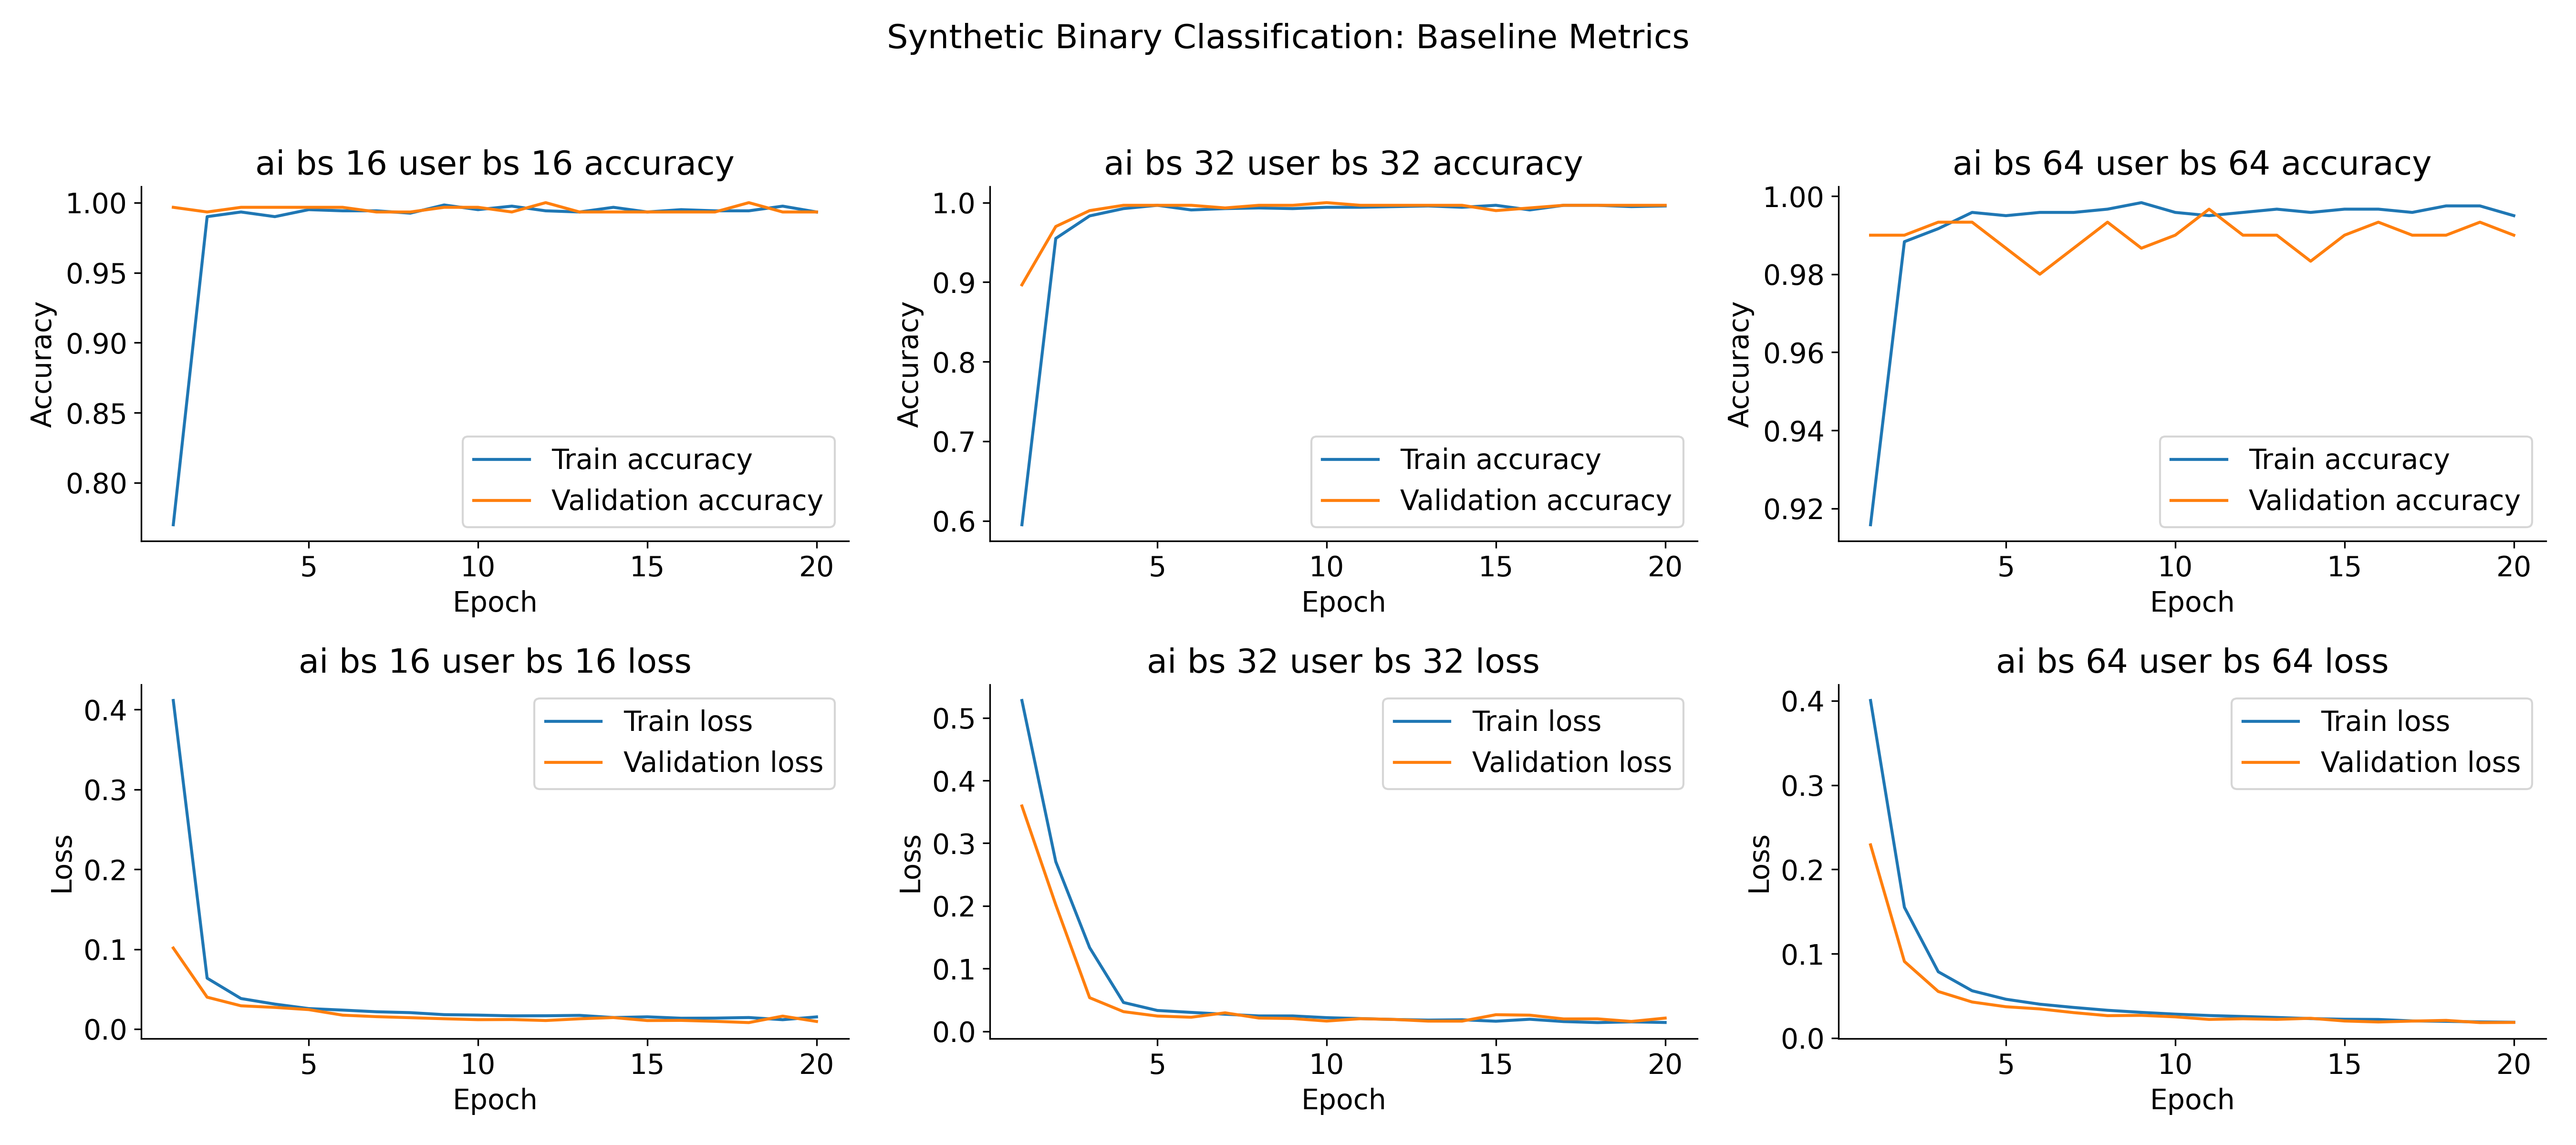
\includegraphics[width=\textwidth]{baseline_metrics.png}
  \caption{Training (solid) and validation (dashed) accuracy (top) and loss (bottom) over 20 epochs for batch sizes 16, 32, and 64. All accuracies stabilize at ≈99\% and losses fall to ≈0 by epoch 5; minor fluctuations (±0.5\%) appear for batch size 64.}
  \label{fig:baseline}
\end{figure}

\subsection{Ablation Studies}
Figure~\ref{fig:ablations} reports two ablations: (a) removal of teacher probability features and (b) soft vs.~hard label inputs. In both cases, training and validation accuracy/loss converge to ≈99\%/≈0, showing these factors do not differentiate interface performance.

\begin{figure}[t]
  \centering
  \subfigure[]{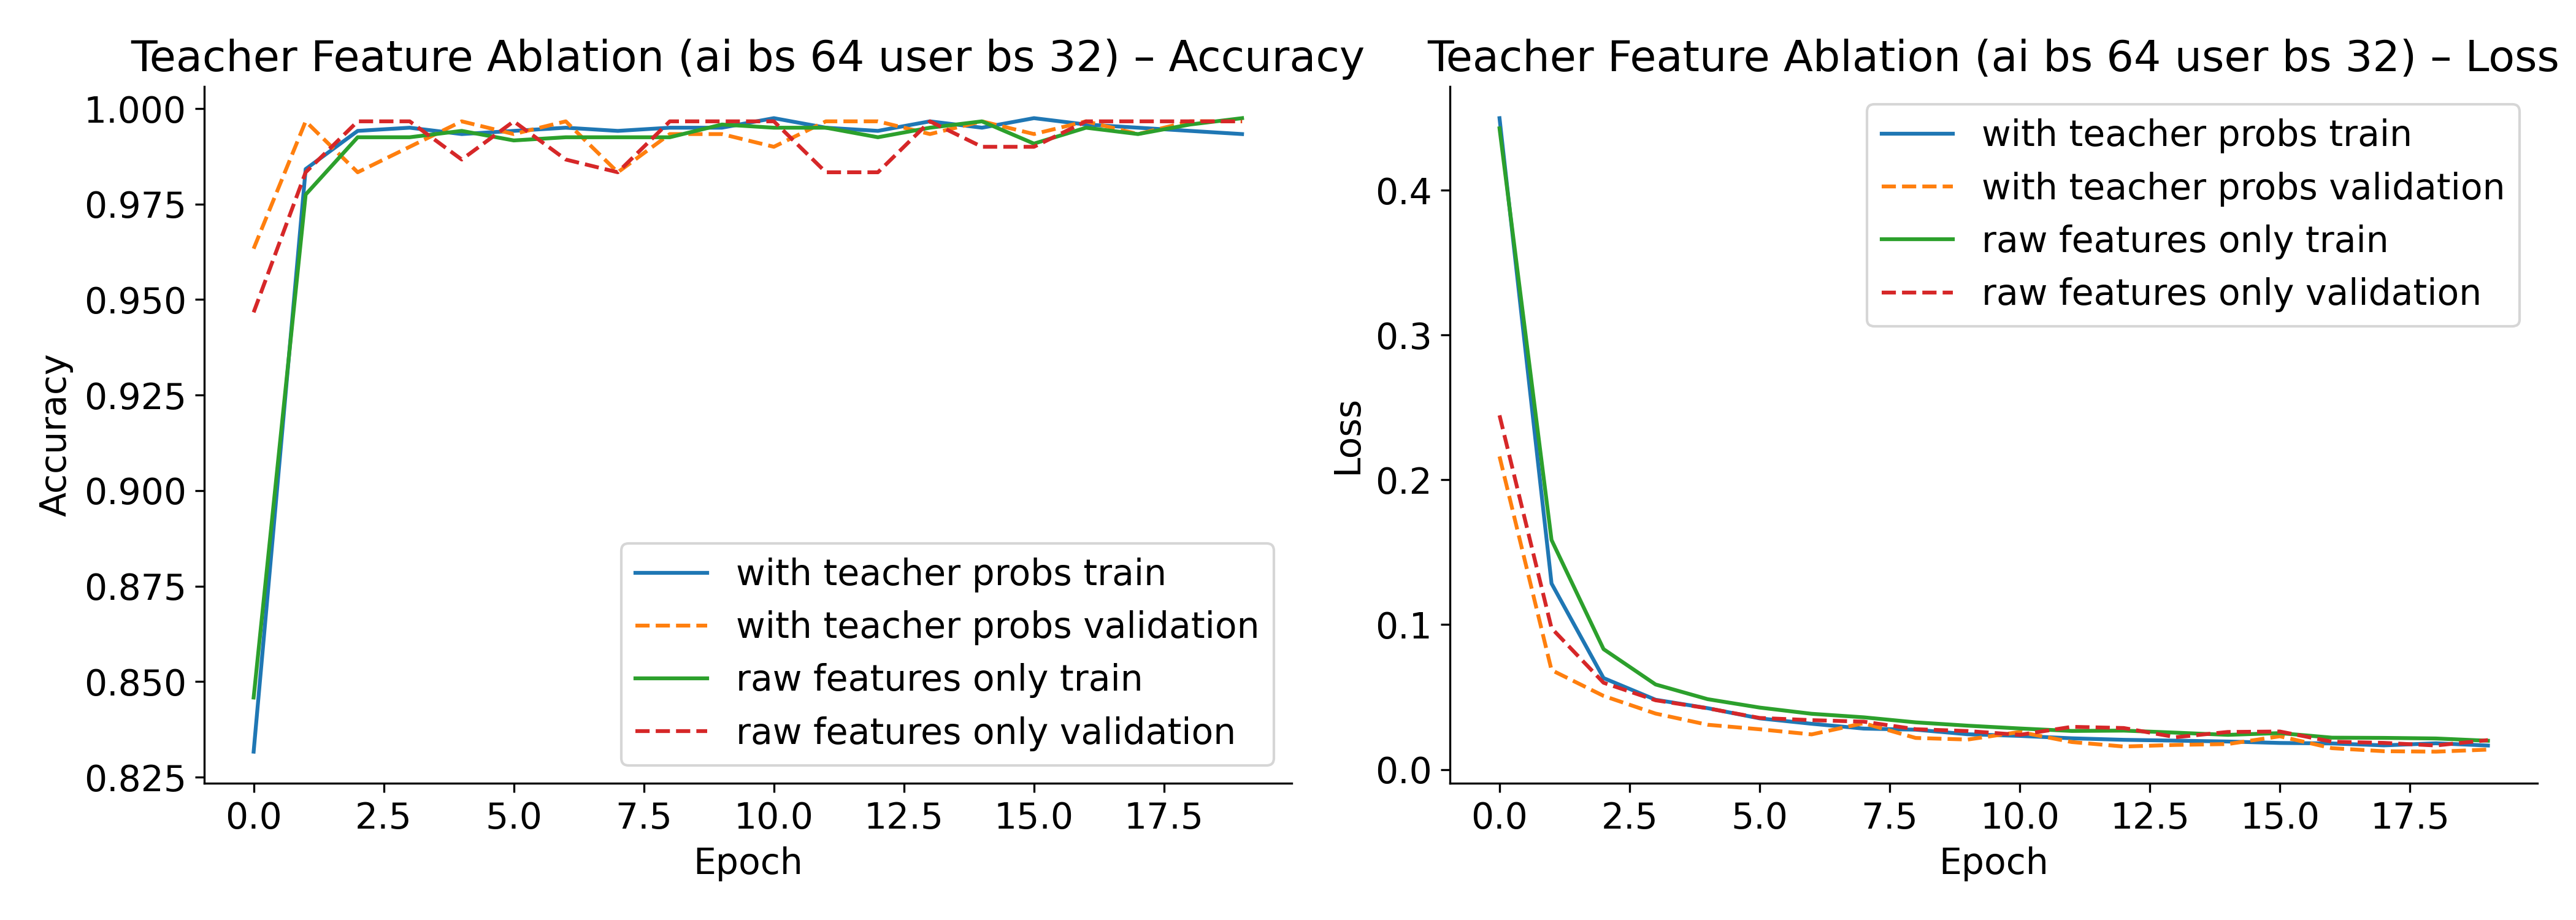
\includegraphics[width=0.48\textwidth]{teacher_feature_ablation.png}}
  \hfill
  \subfigure[]{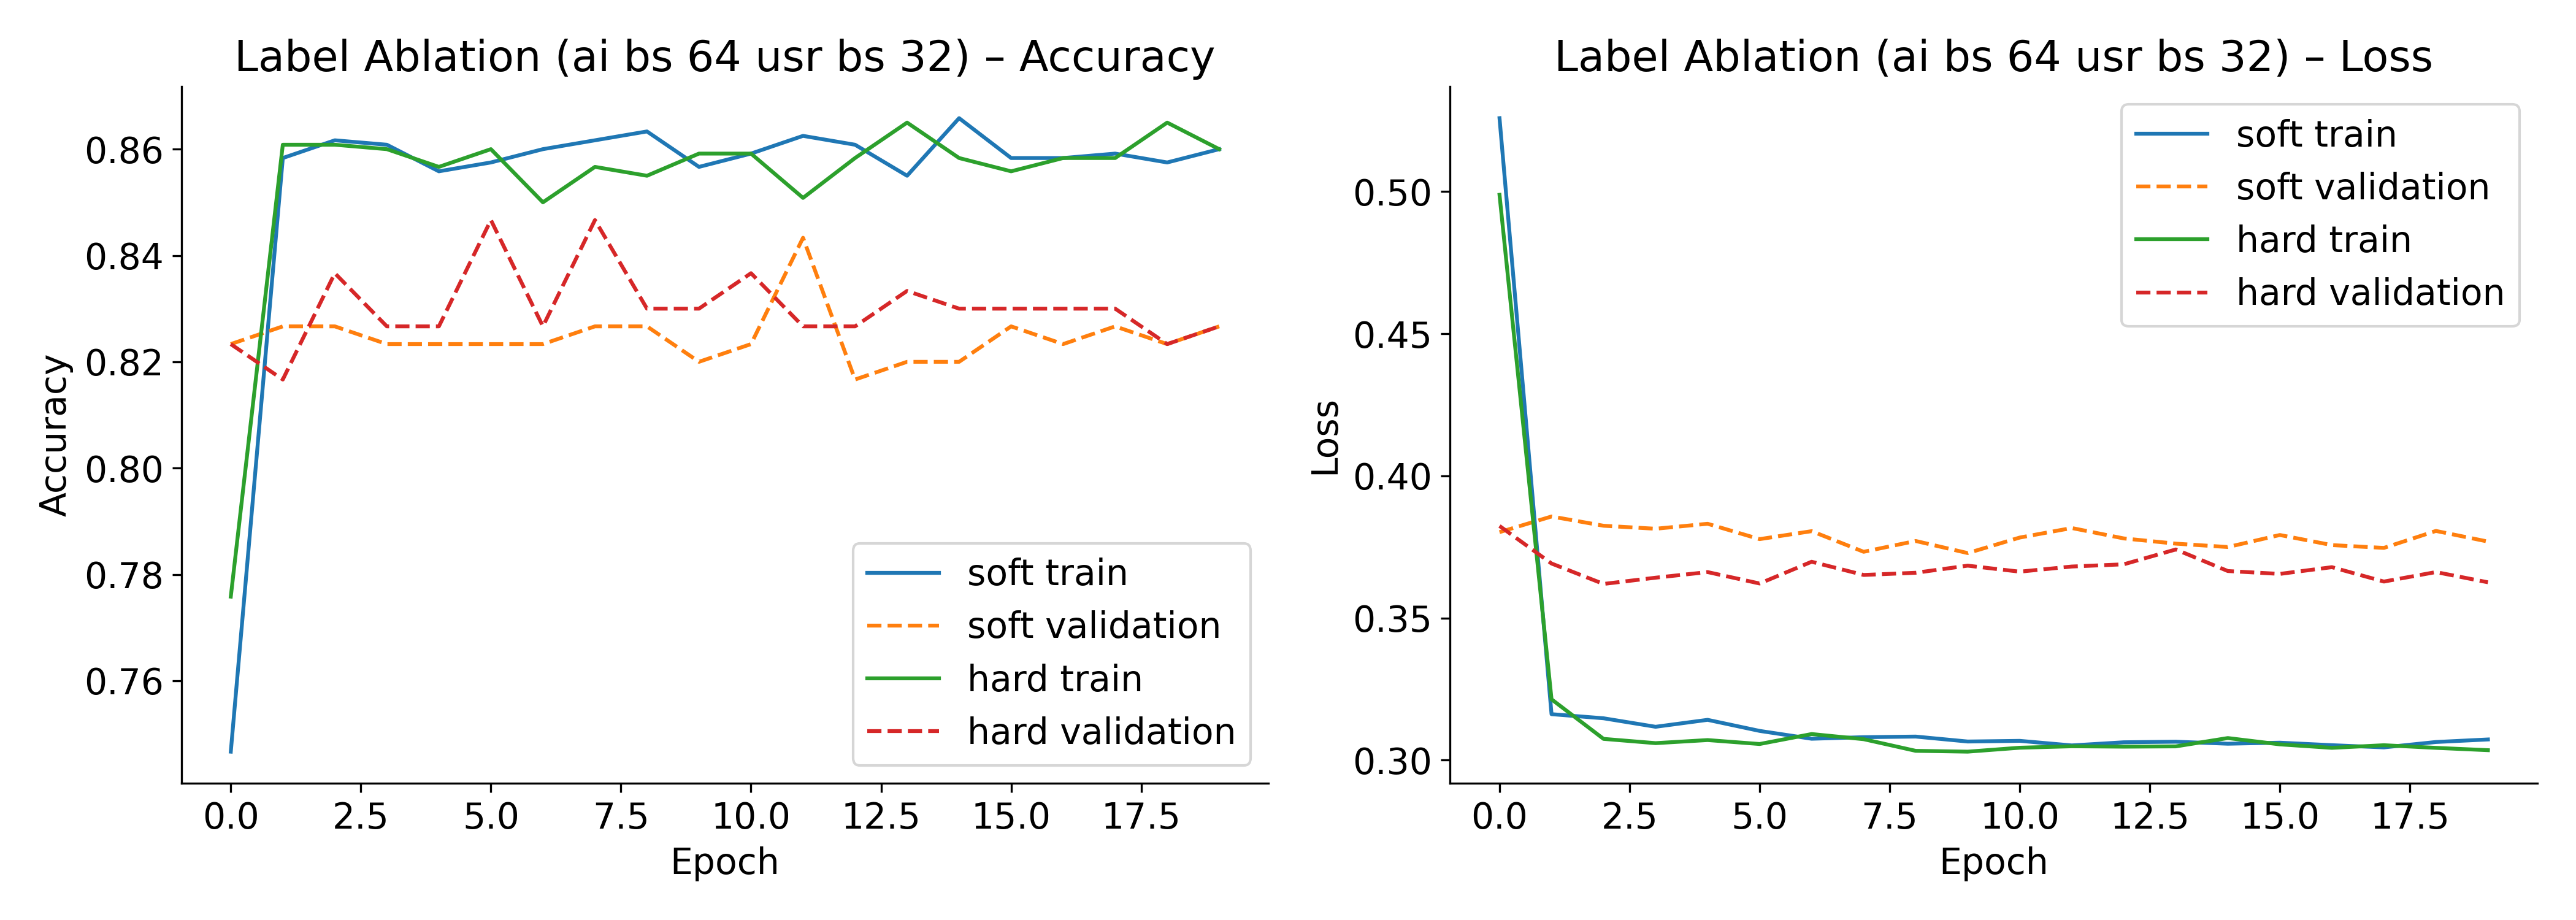
\includegraphics[width=0.48\textwidth]{label_input_ablation.png}}
  \caption{Ablation of (a) teacher probability features and (b) label input type: training (solid) and validation (dashed) accuracy (top) and loss (bottom) over 20 epochs. Both ablations converge to ≈99\% accuracy and ≈0 loss, indicating minimal impact.}
  \label{fig:ablations}
\end{figure}

\subsection{Confidence Threshold Ablation}
Figure~\ref{fig:confidence} shows pseudo-labeling at thresholds 0.6, 0.8, and 0.9: left, training/validation accuracy; middle, losses; right, test accuracy. All thresholds yield ≈100\% training accuracy, validation plateaus at 93–96\%, and test accuracy ≥98\%.

\begin{figure}[t]
  \centering
  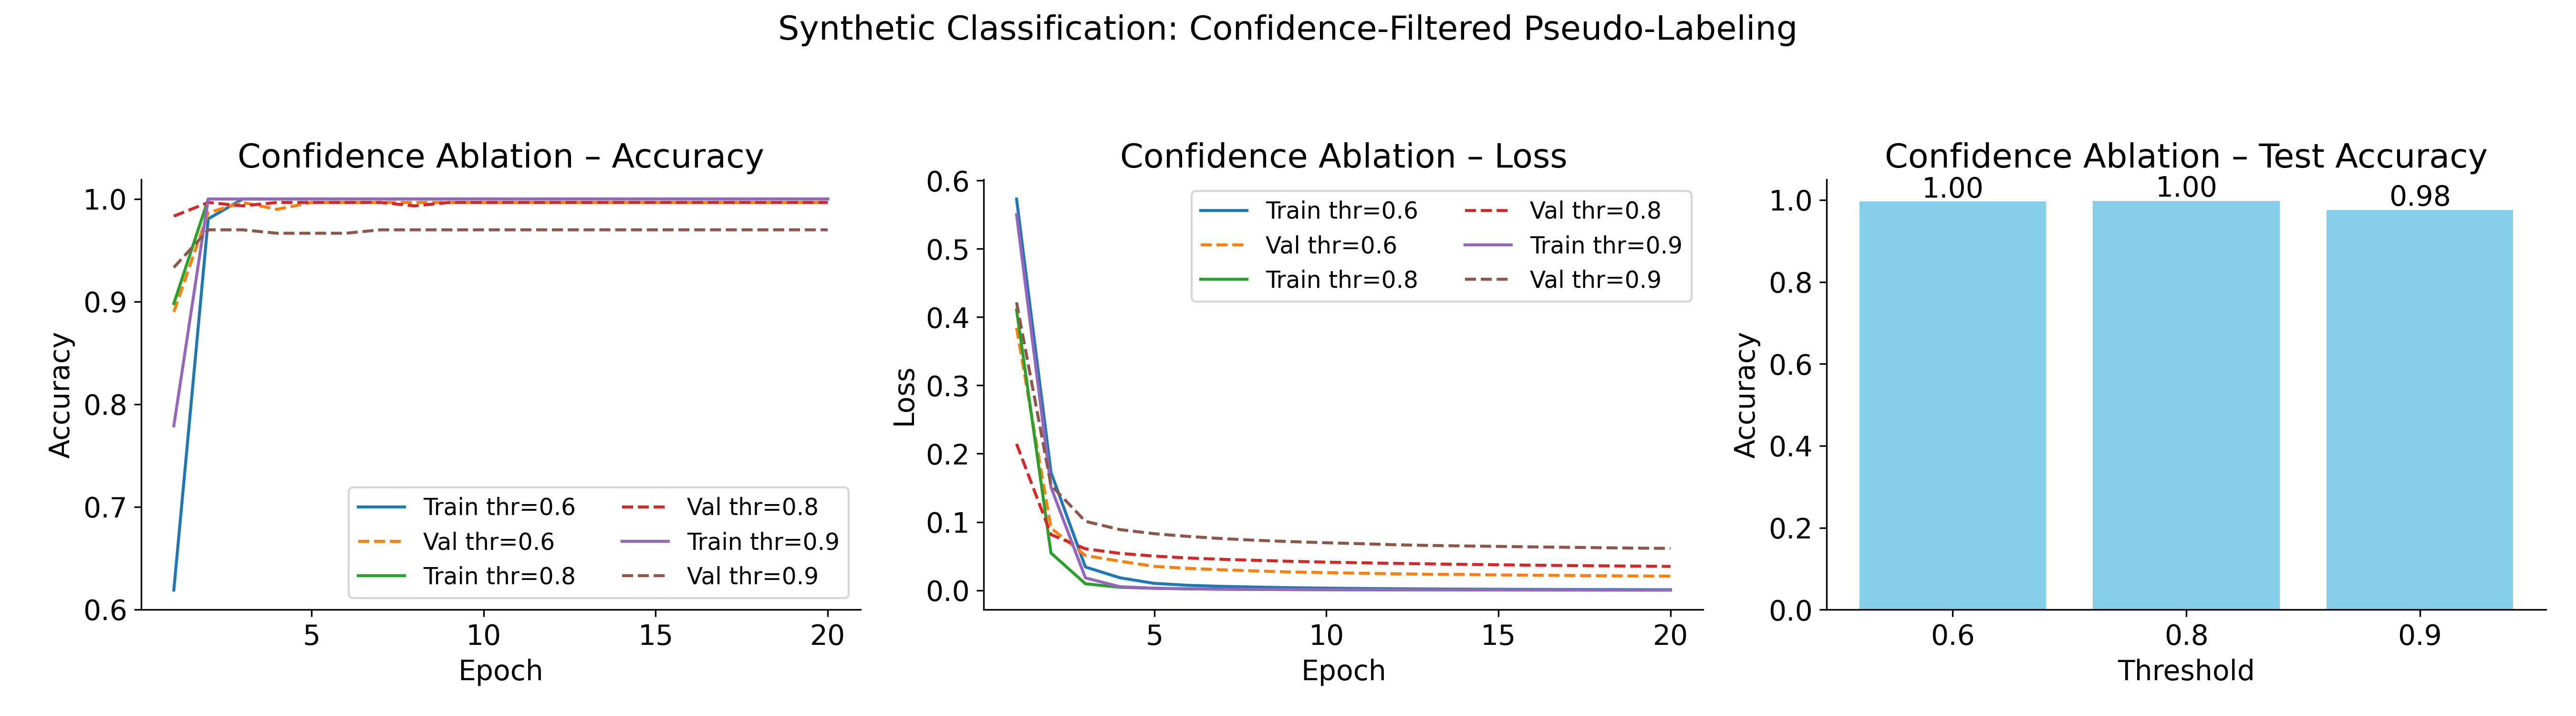
\includegraphics[width=\textwidth]{confidence_ablation_summary.png}
  \caption{Confidence-filtered pseudo-labeling for thresholds 0.6, 0.8, 0.9: (left) training (solid) and validation (dashed) accuracy; (middle) corresponding loss; (right) final test accuracy. All thresholds saturate, showing trivial task difficulty.}
  \label{fig:confidence}
\end{figure}

\subsection{Co-Adaptive Interface Evaluation}
We implemented the dual-channel interface but observed no measurable improvement on any alignment metric compared to static or single-channel variants; all interfaces saturate by epoch 5 (KL divergence →0, trust error →0). Detailed class imbalance and activation-function ablations in the Appendix (\Cref{fig:imbalance,fig:activation}) similarly show negligible effects.

\section{Conclusion}
Our negative results highlight a pitfall: synthetic tasks that saturate simple baselines cannot reveal benefits of co-adaptive explanations. We argue for richer, noisy benchmarks and human-subject studies incorporating cognitive-load measures \citep{sweller1988cognitiveld} and diverse bias profiles to assess whether bias-awareness signals truly improve long-term trust and mental-model alignment.

\bibliography{references}
\bibliographystyle{iclr2025}

\appendix
\section*{Supplementary Material}
\subsection{Class Imbalance Ablation}
\begin{figure}[h]
  \centering
  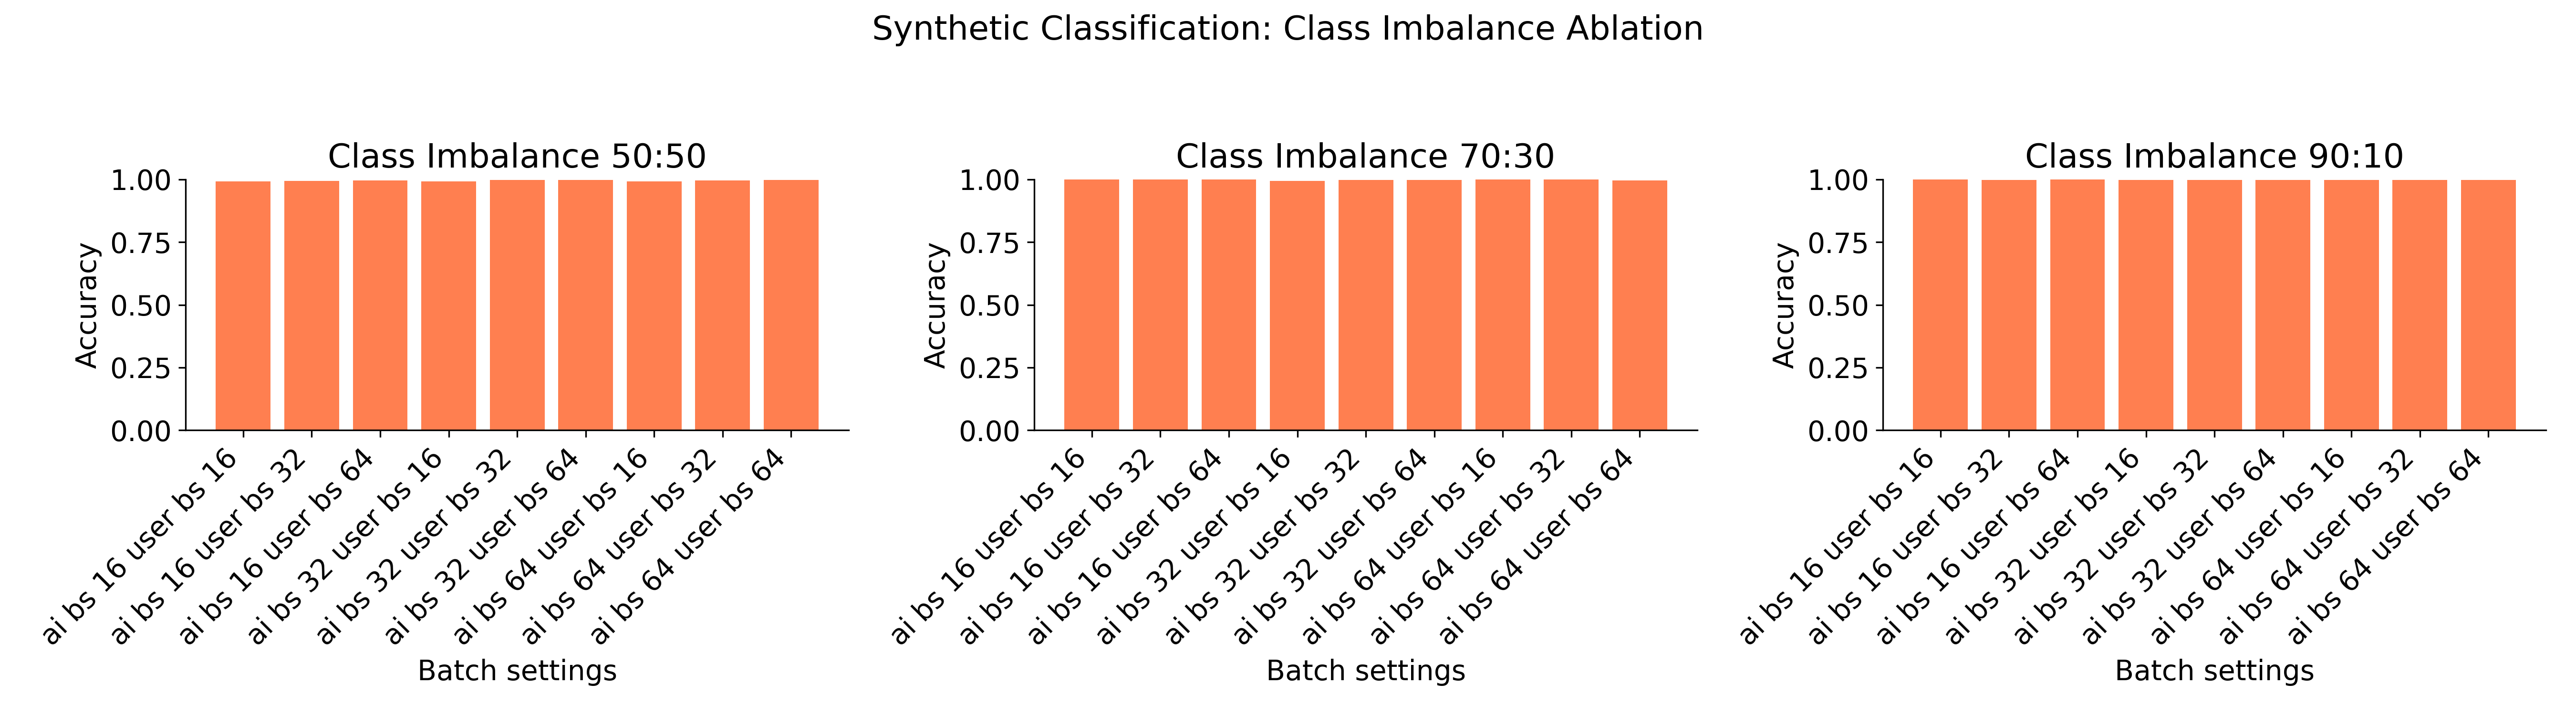
\includegraphics[width=\textwidth]{class_imbalance_ablation.png}
  \caption{Class imbalance ablation: test accuracy across nine batch-size/user-count settings under ratios 50:50, 70:30, 90:10. All configurations yield ≈98–99\%, showing negligible impact of class skew.}
  \label{fig:imbalance}
\end{figure}

\subsection{Activation Function Ablation}
\begin{figure}[h]
  \centering
  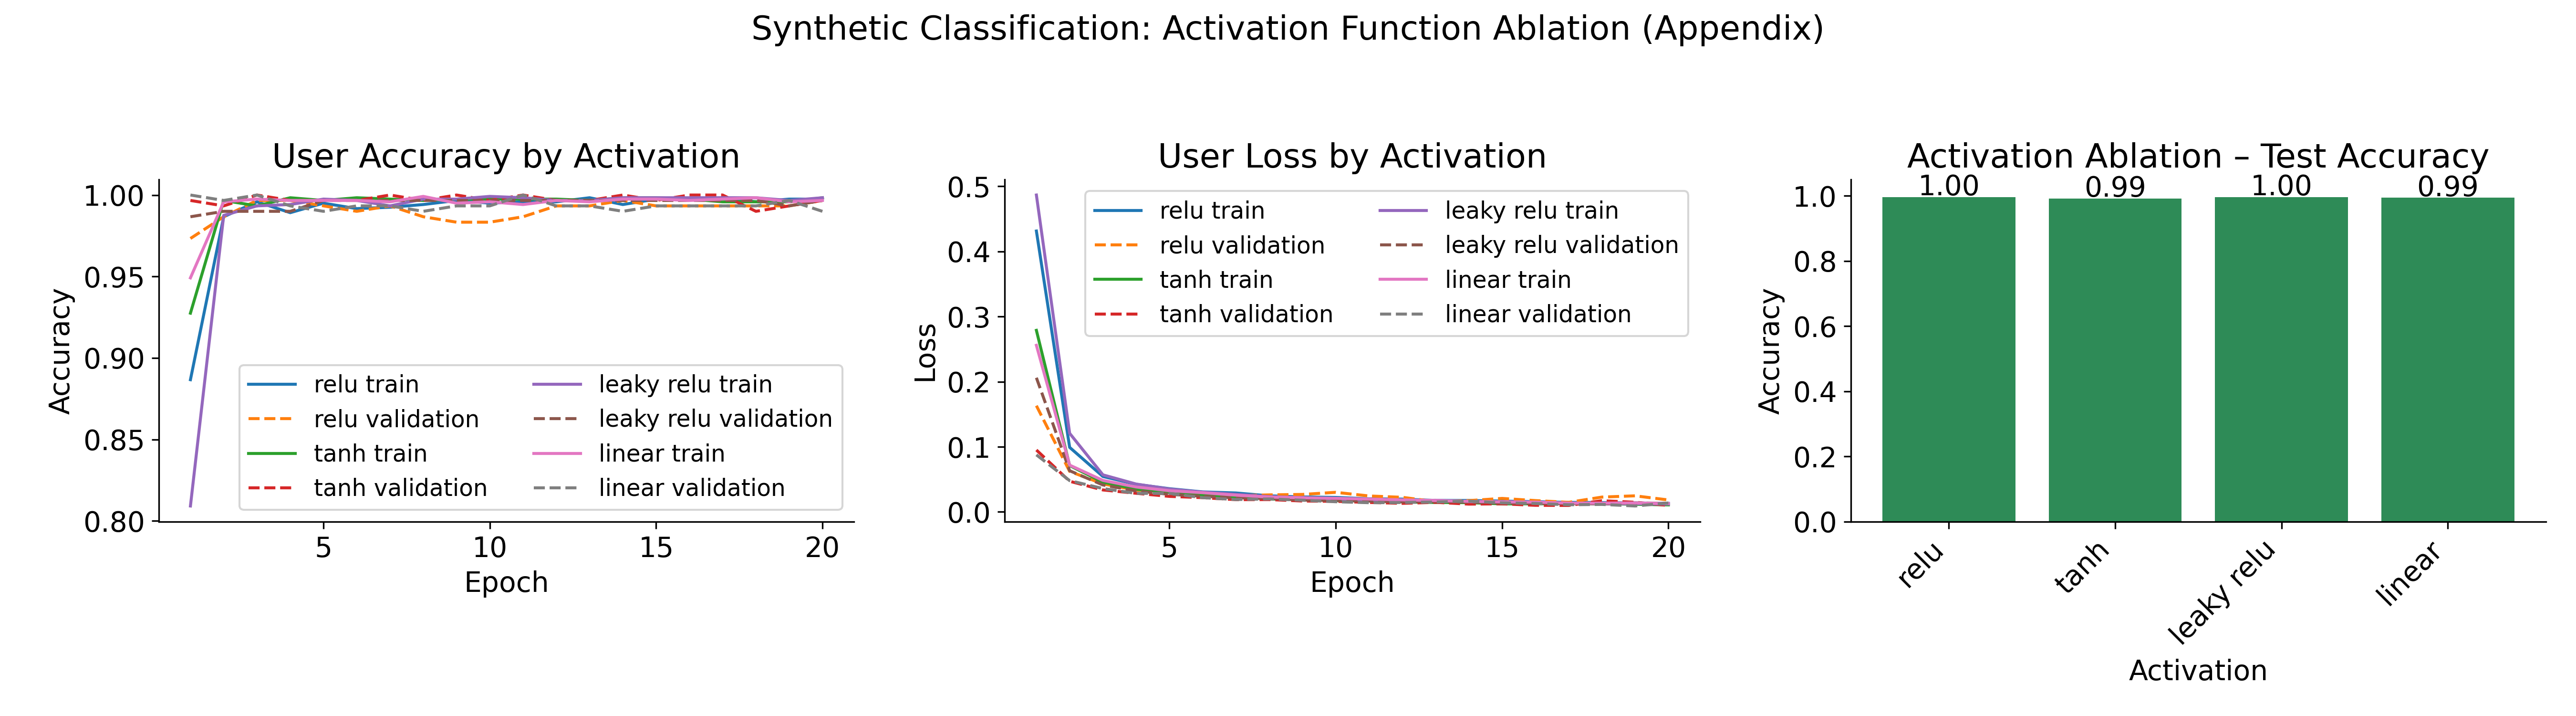
\includegraphics[width=\textwidth]{activation_ablation_appendix.png}
  \caption{Activation ablation: ReLU, Tanh, LeakyReLU, and Linear on the synthetic task. All activations converge to ≈100\% accuracy and near-zero loss by epoch 5; test accuracy differs by ≤1\%.}
  \label{fig:activation}
\end{figure}

\end{document}